% !TEX TS-program = pdflatex
% !TEX encoding = UTF-8 Unicode

% This file is a template using the "beamer" package to create slides for a talk or presentation
% - Giving a talk on some subject.
% - The talk is between 15min and 45min long.
% - Style is ornate.

% MODIFIED by Jonathan Kew, 2008-07-06
% The header comments and encoding in this file were modified for inclusion with TeXworks.
% The content is otherwise unchanged from the original distributed with the beamer package.

%\documentclass[handout]{beamer}
\documentclass{beamer}
\usetheme{metropolis}

\definecolor{vertmoyen}{HTML}{FFFF00}
\definecolor{vertclair}{HTML}{FFFF00}
\definecolor{vertfonce}{HTML}{FFFF00}
\definecolor{deletecol}{HTML}{FF0000}
\definecolor{addcolor} {HTML}{9E0270}

% Copyright 2004 by Till Tantau <tantau@users.sourceforge.net>.
%
% In principle, this file can be redistributed and/or modified under
% the terms of the GNU Public License, version 2.
%
% However, this file is supposed to be a template to be modified
% for your own needs. For this reason, if you use this file as a
% template and not specifically distribute it as part of a another
% package/program, I grant the extra permission to freely copy and
% modify this file as you see fit and even to delete this copyright
% notice. 


\mode<presentation>
{
  \usetheme{Madrid}
  % or ...

 \usecolortheme{dolphin}

  \setbeamercovered{transparent}
  % or whatever (possibly just delete it)
}


\usepackage[english]{babel}
% or whatever

\usepackage[utf8]{inputenc}
% or whatever
\usepackage[normalem]{ulem}

\usepackage{times}
\usepackage[T1]{fontenc}
% Or whatever. Note that the encoding and the font should match. If T1
% does not look nice, try deleting the line with the fontenc.
\usepackage{bussproofs}
\newcommand{\Resolution}[2]{\RightLabel{\footnotesize{$#1$}} \BinaryInfC{$#2$}}

\usepackage[vlined]{algorithm2e}

\usepackage{amsmath}

%\newcommand{\recalltoc}{\frame{\tableofcontents[sectionstyle=show/shaded,subsectionstyle=show/show/hide]}}

\newcommand{\dual}[1]{\ensuremath{\bar{#1}}}
\newcommand{\dn}[2]{#1 \setminus (#2)}
\newcommand{\set}[2]{\ensuremath{\left\{#1\mid#2\right\}}}


\usepackage{tikz}
\usetikzlibrary{positioning}
\usetikzlibrary{decorations, decorations.text,backgrounds}

\tikzstyle{proof edge}=[->,thick,cap=round]
\tikzstyle{deleted edge}=[proof edge, dashed, color=deletecol]

\newcommand{\proofnode}[3][]{
  \node [anchor=mid, #1] (#2) {#3}
}

\newcommand{\rootnode}[1][]{
  \proofnode[#1]{root}{$\bot$}
}

\newcommand<>{\edgewithlabel}[3]{
  \draw#4 [proof edge, color=vertfonce] (#1) -- (#2) node [above, pos=0.3] {\footnotesize #3}
}

\newcommand<>{\drawchildren}[3]{
  \draw#4 [proof edge] (#1) -- (#2);
  \draw#4 [proof edge] (#1) -- (#3)
}

\newcommand{\addchildren}[5]{
  \proofnode[above left  of=#1]{#2}{#3};
  \proofnode[above right of=#1]{#4}{#5}
}

\newcommand{\withchildren}[5]{
  \addchildren{#1}{#2}{#3}{#4}{#5};
  \drawchildren{#1}{#2}{#4}
}

\newcommand<>{\crossnode}[2][]{
  \draw#3 [color=deletecol,thick,cap=round,#1] (#2.mid) ++(10:0.3) -- ++(190:0.6);
}

\newcommand<>{\marknode}[2][.33cm and .29cm]{
  \draw#3 [color=vertclair,line width=1pt] (#2) ellipse (#1);
}
\usepackage{csquotes}
\usepackage{booktabs}
\newenvironment<>{subpart}[1]
{ \begin{block}#2{#1}
  \begin{itemize}
}{
  \end{itemize}
  \end{block}
}


\title[First-Order Partial Regularization] % (optional, use only with long paper titles)
{Partial Regularization of First-Order Resolution Proofs}

%\subtitle{Presentation Subtitle}

\author[Gorzny, Postan, Woltzenlogel Paleo] % (optional, use only with lots of authors)
{J. Gorzny\inst{1} \and E. Postan\inst{2} \and B. Woltzenlogel Paleo\inst{3,4}}
% - Use the \inst{?} command only if the authors have different
%   affiliation.

\institute[] % (optional, but mostly needed)
{
  \inst{1}%
  University of Waterloo
  \and
  \inst{2}
  Universidad Nacional de Rosario
  \and
  \inst{3}%
  Australian National University
  \and
  \inst{4}%
  Vienna University of Technology}
% - Use the \inst command only if there are several affiliations.
% - Keep it simple, no one is interested in your street address.

\date % (optional)
{13 July 2018}

%\subject{Talks}
% This is only inserted into the PDF information catalog. Can be left
% out. 



% If you have a file called "university-logo-filename.xxx", where xxx
% is a graphic format that can be processed by latex or pdflatex,
% resp., then you can add a logo as follows:

 \pgfdeclareimage[height=1cm]{university-logo}{images/GoogleSummer_2014logo}
 \logo{\pgfuseimage{university-logo}}



% Delete this, if you do not want the table of contents to pop up at
% the beginning of each subsection:
%\AtBeginSubsection[]
%{
%  \begin{frame}<beamer>{Outline}
%    \tableofcontents[currentsection,currentsubsection]
%  \end{frame}
%}


% If you wish to uncover everything in a step-wise fashion, uncomment
% the following command: 

%\beamerdefaultoverlayspecification{<+->}


\begin{document}
\def\e{\mbox{\ $\vdash$\ }}

\begin{frame}
  \titlepage
\end{frame}

%\begin{frame}{Outline}
%  \tableofcontents
  % You might wish to add the option [pausesections]
%\end{frame}


% Since this a solution template for a generic talk, very little can
% be said about how it should be structured. However, the talk length
% of between 15min and 45min and the theme suggest that you stick to
% the following rules:  

% - Exactly two or three sections (other than the summary).
% - At *most* three subsections per section.
% - Talk about 30s to 2min per frame. So there should be between about
%   15 and 30 frames, all told.

%\section{Introduction}

%\subsection[Short First Subsection Name]{First Subsection Name}

\begin{frame}{The Quest for Simple Proofs}
\textquote{The 24th problem in my Paris lecture was to be: Criteria of simplicity, or proof of the greatest simplicity of certain proofs. {\color{gray}Develop a theory of the method of proof in mathematics in general. Under a given set of conditions there can be but one simplest proof. Quite generally, if there are two proofs for a theorem, you must keep going until you have derived each from the other, or until it becomes quite evident what variant conditions (and aids) have been used in the two proofs. }}\\
\hspace{8cm}--David Hilbert \cite{thiele2003hilbert}

\end{frame}

\begin{frame}{First-Order Proof Compression Motivation}
%an accessible, good motivational example for proof compression
\begin{itemize}
\item The best, most efficient provers, do not generate the best, least redundant proofs.\vspace{1cm}
\item Many compression algorithms for propositional proofs; few for first-order proofs. \vspace{1cm}
\item Finding a minimal proof is NP-hard, so use heuristics to find smaller proofs (see \cite{fontaine2011compression})
\end{itemize}
\end{frame}

\begin{frame}{The `Real World'}
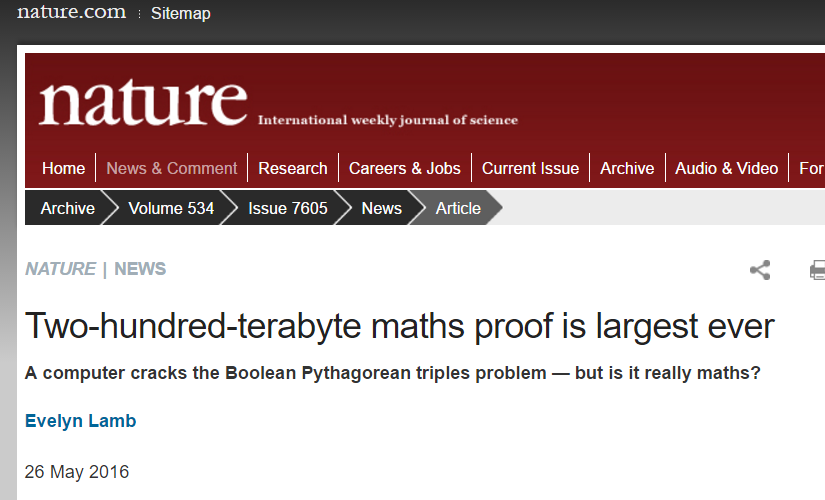
\includegraphics[scale=0.7]{images/nature.png}\\
{\color{gray} (See \cite{DBLP:journals/corr/HeuleKM16})}
\end{frame}


\begin{frame}{Proofs as Interfaces}
\begin{itemize}
\item Larger proofs harder/longer to check; use more resources\\ ~\
\item Proofs that are too large may mean solutions can't be written (SAT 2014)\\ ~\
\item May use a strict subset of original hypothesis: better proofs!
\end{itemize}
\end{frame}




\begin{frame}{Our Goal}

Lifting propositional proof compression algorithms to first-order logic.\\
\vspace{1cm}
Previous work: \texttt{LowerUnits} \cite{fontaine2011compression}.\\
\vspace{1cm}
This work: \texttt{RecyclePivotWithIntersection} \cite{fontaine2011compression, bar2008linear}

\end{frame}




%{
  \setbeamercolor{background canvas}{bg=lightgray}
\begin{frame}{(Propositional) Proofs}
%introduction to proofs as we're going to see them, ideally formally and with a small example

\begin{definition}[Proof]
A directed acyclic graph $\langle V,E,\Gamma \rangle$, where
\begin{itemize}
\item $V$ is a set of nodes
\item $E$ is a set of edges labeled by literals
\item $\Gamma$ (the proof clause) is inductively constructible using \emph{axiom} and \emph{resolution} nodes
\end{itemize}
\end{definition}

\begin{definition}[Axiom]
A proof with a single node (so $E=\emptyset$)
\end{definition}
\end{frame}
}

{
  \setbeamercolor{background canvas}{bg=lightgray}
\begin{frame}{(Propositional) Resolution}
%a quick introduction to resolution, with a small propositional example
\begin{definition}[Resolution]
Given two proofs $\psi_L$ and $\psi_R$ with conclusions $\Gamma_L$ and $\Gamma_R$ with some literal $l$ such that $\overline{l}\in \Gamma_L$ and $l\in \Gamma_R$, the resolution proof $\psi$ of $\psi_L$ and $\psi_R$ on $l$, denoted $\psi=\psi_L \psi_R$ is such that:
\begin{itemize}
\item $\psi$'s nodes are the union of the nodes of $\psi_L$ and $\psi_R$, and a new root node
\item there is an edge from $\rho(\psi)$ to $\rho(\psi_L)$ labeled with $\overline{l}$
\item there is an edge from $\rho(\psi)$ to $\rho(\psi_R)$ labeled with $l$
\item $\psi$'s conclusion is $(\Gamma_L\setminus\{\overline{l}\})\cup(\Gamma_R\setminus\{l\})$
\end{itemize}
\end{definition}
\end{frame}
}
%\begin{frame}{A Propositional Proof}
%a small example to illustrate the definitions from the last two slides\\
%the example should be redundant, so that we can show it again after the next slide in it's more minimal state\\
%ideally minimized via LU, so that we can show the transformation later
      \centering
      \begin{tikzpicture}[node distance=1.2cm]
        \rootnode;
        \withchildren{root} {r9}{\dual{c}}  {r6}{c};
     \proofnode[above left of=r9] {r8} {a,\dual{c}};
     \proofnode[above of=r8] {r7} {a,\dual{b},\dual{c}};
     \proofnode[above right of=r6] {r5} {a,c};

        \withchildren{r5}  {r4}{b} {r2}{a,\dual{b},c};
        \withchildren{r4}   {r1}{\dual{a}} {r3}{a,b};
        \drawchildren {r6} {r1} {r5};
      \draw[proof edge] (r9) -- (r1);
      \draw[proof edge] (r9) -- (r1);
      \draw[proof edge] (r9) -- (r8);
      \draw[proof edge] (r8) -- (r7);
      \draw[proof edge] (r8) -- (r4);
      \end{tikzpicture}
\end{frame}

%{

\begin{frame}{Deletion}
%how deleting subproofs or edges in proofs affect them
Deletion of an edge\\
\begin{itemize}
\item The resolvent is replaced by the other premise
\item Some subsequent resolutions may have to be deleted too
\end{itemize}
\vspace{1cm}
Deletion of a subproof $\psi$\\
\begin{itemize}
\item Deletion of every edge coming to $\rho(\psi)$
\item The operation is commutative and associative
\end{itemize}
\end{frame}
}

%{
%  \setbeamercolor{background canvas}{bg=lightgray}
%\begin{frame}{Redundancy}
%types of redundancy we hope to remove, small examples (before/after proofs; not animated)
%\end{frame}
%}

{

\begin{frame}{First-Order Proofs}
%key differences from propositional case; example of first-order proofs
\begin{definition}[First-Order Proof]
A directed acyclic graph $\langle V,E,\Gamma \rangle$, where
\begin{itemize}
\item $V$ is a set of nodes
\item $E$ is a set of edges labeled by literals {\bf and substitutions}
\item $\Gamma$ (the proof clause) is inductively constructible using \emph{axiom}, {\bf\emph{(first-order) resolution}}, {\bf and \emph{contraction}} nodes
\end{itemize}
\end{definition}
\vspace{0.5cm}
Axioms are unchanged
\end{frame}
}

{

\begin{frame}{Substitutions and Unifiers}
\begin{definition}[Substitution]
A mapping $\{X_1\setminus t_1, X_2\setminus t_2,\ldots\}$ from variables $X_1,X_2,\ldots$ to terms $t_1,t_2,\ldots$
\end{definition}

%example here

\begin{definition}[Unifier]
A substitution that makes two terms equal when applied to them.
\end{definition}

%example here
\end{frame}
}



\begin{frame}{First-Order (Unifying) Resolution}
%definition (incl. mgu); ?
%example of unifying resolution ?
\begin{definition}[First-Order Resolution]
Given two proofs $\psi_L$ and $\psi_R$ with conclusions $\Gamma_L$ and $\Gamma_R$ with some literal $l$ such that $l_L\in \Gamma_L$ and $l_R\in \Gamma_R$, and $\sigma_L$ and $\sigma_R$ are substitutions usch that $l_L\sigma_L=\overline{l_R}\sigma_R$, and the variables in $(\Gamma_L\setminus l_L)\sigma_L$ and $(\Gamma_R\setminus l_R)\sigma_R$ are disjoint, then the resolution proof $\psi$ of $\psi_L$ and $\psi_R$ on $l$, denoted $\psi=\psi_L \psi_R$ is such that:
\begin{itemize}
\item $\psi$'s nodes are the union of the nodes of $\psi_L$ and $\psi_R$, and a new root node
\item there is an edge from $\rho(\psi)$ to $\rho(\psi_L)$ labeled with $l_L$ and $\sigma_L$
\item there is an edge from $\rho(\psi)$ to $\rho(\psi_R)$ labeled with $l_R$ and $\sigma_R$
\item $\psi$'s conclusion is $(\Gamma_L\setminus l_L)\sigma_L\cup (\Gamma_R\setminus l_R)\sigma_R$
\end{itemize}
\end{definition}
\end{frame}

\begin{frame}{Unifying Resolution Example}
\begin{center}
      \begin{tikzpicture}[node distance=2cm]
 \proofnode[above left of=root] {n1} {$\eta_1$: $p(a)\e$};
 \proofnode[above right of=root] {n2} {$\eta_2$: $q(Y, X) \e p(Y)$};
 \proofnode{root} {$\psi$: $q(a,X)\e $};
 
       \draw[proof edge] (root) -- (n2);
       
             \draw[proof edge] (root) -- (n1);
 \end{tikzpicture}\\\vspace{1cm}
 $\sigma = \{Y\rightarrow a\}$\\
 Refutation when $\psi=\bot$
 \end{center}
\end{frame}


%\begin{frame}{Contraction}
%definition; small example
\begin{definition}[Contraction]
If $\psi'$ is a proof and $\sigma$ is a unifier of $\{l_1,\ldots,l_n\}\subset \Gamma'$, then a contraction $\psi$ is a proof where
\begin{itemize}
\item $\psi$'s nodes are the union of the nodes of $\psi'$ and a new node $v$
\item There is an edge from $\rho(\psi')$ to $v$ labeled with $\{l_1,\ldots,l_n\}$ and $\sigma$
\item The conclusion is $(\Gamma'\setminus \{l_1,\ldots,l_n\})\sigma \cup \{l\}$, where $l=l_k\sigma$ for $k\in \{1,\ldots,n\}$
\end{itemize}
\end{definition}
\end{frame}

\begin{frame}{Contraction Example}
\only<1>{
\begin{center}
      \begin{tikzpicture}[node distance=2cm]
 \proofnode[above of=root] {n1} {$\eta_1$: $p(X,Y), p(a,Z), p(a,f(b)) \e q(Z)$};
 \proofnode{root} {$\psi$: $p(a,f(b))\e q(f(b))$};
 
             \draw[proof edge] (root) -- (n1);
 \end{tikzpicture}\\\vspace{1cm}
 $\sigma = \{X\rightarrow a, Y\rightarrow f(b), Z\rightarrow f(b)\}$\\
 \end{center}
 }
 \only<2>{
 \begin{center}
      \begin{tikzpicture}[node distance=2cm]
 \proofnode[above of=root] {n1} {$\eta_1$: $p(X,Y), p(X,Z), p(U,V) \e q(Z)$};
 \proofnode{root} {$\psi$: $p(X,Z)\e q(Z)$};
 
             \draw[proof edge] (root) -- (n1);
 \end{tikzpicture}\\\vspace{1cm}
 $\sigma = \{Y\rightarrow Z, U\rightarrow Z, V\rightarrow Z\}$\\
 \end{center}
 }
 \only<3>{
 \begin{center}
      \begin{tikzpicture}[node distance=2cm]
 \proofnode[above of=root] {n1} {$\eta_1$: $p(X,Y), p(a,Z), p(a,f(b)) \e q(Z)$};
 \proofnode{root} {$\psi$: $p(X,Y), p(a,f(b))\e q(f(b))$};
 
             \draw[proof edge] (root) -- (n1);
 \end{tikzpicture}\\\vspace{1cm}
 $\sigma = \{Z\rightarrow f(b)\}$\\
 \end{center}
 }
\end{frame}


%\section{RPI}

\begin{frame}{Recycling Pivots}
Removes \emph{irregularities}: inferences $\eta$ where the pivot occurs as a pivot of another inference below $\eta$ on the path to the root\\
\begin{itemize}
\item Store a set of \emph{safe} $\mathcal{S}(\eta)$ literals for each node $\eta$
\end{itemize}


\pause
\begin{itemize}
\item If there are multiple paths, take \emph{intersection} of safe literals
\end{itemize}
\pause
\begin{itemize}
\item Bottom-up: compute safe literals; mark deletions
\item Top-down: regularize
\end{itemize}
\end{frame}

\begin{frame}{Regularization Can Be Bad}
Resolution without irregularities is still complete. But:

\begin{theorem}[\cite{tseitin1970complexity}]
There are unsatisfiable formulas whose shortest regular resolution refutations are exponentially longer than their shortest unrestricted resolution refutations.
\end{theorem}
\end{frame}

\begin{frame}{Propositional Example}
%quick, clear example of LU (animated), perhaps showing how one of the redundancies described before is fixed
\begin{columns}
\column{0.5\textwidth}
      \begin{center}
      \begin{tikzpicture}[node distance=1.2cm]
        \rootnode;
        \withchildren{root} {r9}{b}  {r6}{\dual{b}};
         \withchildren{r6} {r1}{\dual{a}}  {r2}{a\dual{b}};
                  \withchildren{r1} {r3}{\dual{b}}  {r4}{\dual{a}b};
  %   \proofnode[above left of=r9] {r8} {a,\dual{c}};
       % \drawchildren {r6} {r1} {r5};
      %\draw[proof edge] (r9) -- (r1);
      \end{tikzpicture}
\end{center}
\column{0.5\textwidth}
  \only<1-5>{
      \begin{center}

      \begin{tikzpicture}[node distance=1.2cm]
        \rootnode;
        \proofnode[above left of=root]{r9}{b};
        \proofnode[above right of=root] {r6}{\dual{b}};
         \proofnode[above left of=r6]{r1}{\dual{a}};
         \proofnode[above right of=r6] {r2}{a\dual{b}};
          \proofnode[above left of=r1] {r3}{\dual{b}};
    \proofnode[above right of=r1] {r4}{\dual{a}b};
      \draw[proof edge] (root) -- (r9);
            \draw[proof edge] (root) -- (r6);
                  \draw[proof edge] (r6) -- (r1);
                        \draw[proof edge] (r6) -- (r2);
                              \draw[proof edge] (r1) -- (r3);
                                                            \draw[proof edge] (r1) -- (r4);

\proofnode[left of=r9]{ra}{\alt<-1>{\color{white}$\{b\}$}{$\{b\}$}};
\proofnode[right of=r6]{rb}{\alt<-1>{\color{white}$\{\dual{b}\}$}{$\{\dual{b}\}$}};

\proofnode[left of=r1]{rc}{\alt<-2>{\color{white}$\{\dual{a}\dual{b}\}$}{$\{\dual{a}\dual{b}\}$}};
\proofnode[right of=r2]{rd}{\alt<-2>{\color{white}$\{a\dual{b}\}$}{$\{a\dual{b}\}$}};

\proofnode[left of=r3]{re}{\alt<-3>{\color{white}$\{\dual{a}b\dual{b}\}$}{$\{\dual{a}{\color{red}\dual{b}}\}$}};
\proofnode[right of=r4]{rf}{\alt<-3>{\color{white}$\{ab\}$}{$\{ab\}$}};
\crossnode<5>{r4};
\marknode<5>{r1};
      \end{tikzpicture}\\
      $\uparrow$ safe literal collection
\end{center}
}
  \only<6>{
      \begin{center}

      \begin{tikzpicture}[node distance=1.2cm]
        \rootnode;
        \proofnode[above left of=root]{r9}{b};
        \proofnode[above right of=root] {r6}{b};

         \proofnode[above right of=r6] {r2}{a\dual{b}};

    \proofnode[above left of=r6] {r4}{\dual{b}};
      \draw[proof edge] (root) -- (r9);
            \draw[proof edge] (root) -- (r6);
                        \draw[proof edge,color=red] (r6) -- (r2);

                                                            \draw[proof edge, color=red] (r6) -- (r4);
\crossnode<6>{r2};
\crossnode<6>{r6};

      \end{tikzpicture}\\
      $\downarrow$ regularization
\end{center}

}
  \only<7>{
      \begin{center}
      \begin{tikzpicture}[node distance=1.2cm]
        \rootnode;
        \proofnode[above left of=root]{r9}{b};
    \proofnode[above right of=root] {r4}{\dual{b}};
      \draw[proof edge] (root) -- (r9);
            \draw[proof edge] (root) -- (r4);

      \end{tikzpicture}\\
$\downarrow$ regularization
\end{center}

}


\end{columns}
\end{frame}

\begin{frame}{Pre-Regularization Checks I}



\only<1>{
      \begin{center}

      \begin{tikzpicture}[node distance=1cm]
        \rootnode;
        \proofnode[above left=0cm and 0.5cm of root]{r9}{$\eta_6$: $p(Y,b)\vdash$};
        \proofnode[above right=0cm and 0.5cm of root] {r6}{$\eta_5$: $\vdash p(a,X)$};
         \proofnode[above left=1cm and 1.5cm of r6]{r1}{$\eta_3$: $\vdash q(c)$};
         \proofnode[above right=1cm and -1.5cm of r6] {r2}{$\eta_4$: $q(c) \vdash p(a,X)$};
          \proofnode[above left=1cm and -2cm of r1] {r3}{$\eta_1$: $\vdash p(W,X)$\hspace{3cm}};
    \proofnode[above right=1cm and 1cm of r1] {r4}{$\eta_2$: $p(W,X) \vdash q(c)$};
      \draw[proof edge] (root) -- (r9);
            \draw[proof edge] (root) -- (r6);
                  \draw[proof edge] (r6) -- (r1);
                        \draw[proof edge] (r6) -- (r2);
                              \draw[proof edge] (r1) -- (r3);
                                                            \draw[proof edge] (r1) -- (r4);

{\color{darkgray}
\proofnode[below left=0 and -0.5cm of r9]{ra}{$\{  p(Y,b) \vdash \}$};
\proofnode[below right=0 and -0.5cm of r6]{rb}{$\{\vdash p(a,X) \}$};

\proofnode[below left=0 and -0.5cm of r1]{rc}{$\{\vdash q(c), p(a,X)\}$};
\proofnode[below right=0 and -1.5cm of r2]{rd}{$\{q(c) \vdash p(a,X) \}$};

\proofnode[below left=0 and -1cm of r3]{re}{\color{black}$\{ \vdash q(c),$ {\color{red}$p(a,X)$} $\}$};
\proofnode[below right=0 and -1.5cm of r4]{rf}{$\{p(W,X) \vdash q(c), p(a,X)\}$};
}

      \end{tikzpicture}\\
      $\sigma = \{W\rightarrow a\} \implies \sigma\eta_1 \in \mathcal{S}(\eta_1)$
   \end{center}
   }
   \only<2>{
        \begin{center}

      \begin{tikzpicture}[node distance=1cm]
        \rootnode;
        \proofnode[above left=0cm and 0.5cm of root]{r9}{$\eta_6$: $p(Y,b)\vdash$};
        \proofnode[above right=0cm and 0.5cm of root] {r6}{$\eta_1$: $\vdash p(W,X)$};

      \draw[proof edge] (root) -- (r9);
            \draw[proof edge] (root) -- (r6);



      \end{tikzpicture}\\
            $\sigma = \{W\rightarrow Y, X \rightarrow b\}$
      \end{center}
   }
\end{frame}

\begin{frame}{Pre-Regularization Checks II}



\only<1>{
      \begin{center}

      \begin{tikzpicture}[node distance=1cm]
        \rootnode;
        \proofnode[above left=0cm and 0.5cm of root]{r9}{$\eta_6$: $p(Y,b)\vdash$};
        \proofnode[above right=0cm and 0.5cm of root] {r6}{$\eta_5$: $\vdash p(a,X)$};
         \proofnode[above left=1cm and 1.5cm of r6]{r1}{$\eta_3$: $\vdash q(c)$};
         \proofnode[above right=1cm and -1.5cm of r6] {r2}{$\eta_4$: $q(c) \vdash p(a,X)$};
          \proofnode[above left=1cm and -2cm of r1] {r3}{$\eta_1$: $\vdash p(W,c)$\hspace{3cm}};
    \proofnode[above right=1cm and 1cm of r1] {r4}{$\eta_2$: $p(W,X) \vdash q(c)$};
      \draw[proof edge] (root) -- (r9);
            \draw[proof edge] (root) -- (r6);
                  \draw[proof edge] (r6) -- (r1);
                        \draw[proof edge] (r6) -- (r2);
                              \draw[proof edge] (r1) -- (r3);
                                                            \draw[proof edge] (r1) -- (r4);

{\color{darkgray}
\proofnode[below left=0 and -0.5cm of r9]{ra}{$\{  p(Y,b) \vdash \}$};
\proofnode[below right=0 and -0.5cm of r6]{rb}{$\{\vdash p(a,X) \}$};

\proofnode[below left=0 and -0.5cm of r1]{rc}{$\{\vdash q(c), p(a,X)\}$};
\proofnode[below right=0 and -1.5cm of r2]{rd}{$\{q(c) \vdash p(a,X) \}$};

\proofnode[below left=0 and -1cm of r3]{re}{\color{black}$\{ \vdash q(c),$ {\color{red}$p(a,X)$} $\}$};
\proofnode[below right=0 and -1.5cm of r4]{rf}{$\{p(W,X) \vdash q(c), p(a,X)\}$};
}

      \end{tikzpicture}\\
      $\sigma = \{W\rightarrow a, X\rightarrow c\} \implies \sigma\eta_1 \in \mathcal{S}(\eta_1)$\\
      \alert{but...}
   \end{center}
   }
   \only<2>{
        \begin{center}

      \begin{tikzpicture}[node distance=1cm]
        \rootnode;
        \proofnode[above left=0cm and 0.5cm of root]{r9}{$\eta_6$: $p(Y,b)\vdash$};
        \proofnode[above right=0cm and 0.5cm of root] {r6}{$\eta_1$: $\vdash p(c,a)$};

      \draw[proof edge] (root) -- (r9);
            \draw[proof edge] (root) -- (r6);
\crossnode{root};

      \end{tikzpicture}\\
      \vspace{2cm}
            no $\sigma$!\\
      \end{center}
   }
\end{frame}

\begin{frame}{Pre-Regularization Unifiability}
\begin{definition}
Let $\eta$ be a node with pivot $\ell'$ unifiable with safe literal $\ell$ which is resolved against literals $\ell_1$, \ldots, $\ell_n$ in a proof $\psi$. $\eta$ is said to satisfy the \emph{pre-regularization unifiability property} in $\psi$ if $\ell_1$,\ldots,$\ell_n$, and $\dual{\ell'}$ are unifiable.
\end{definition}
\end{frame}

\begin{frame}{Post-Regularization Checks}
\only<1>{
\begin{center}
      \begin{tikzpicture}[node distance=1cm]
        \rootnode;
        \proofnode[above left=0.5cm and 0.5cm of root]{r8}{$\eta_8$: $q(f(a,e),c)\vdash$};
        \proofnode[above right=0.5cm and 0.5cm of root] {r7}{$\eta_7$: $\vdash q(f(a,Z),c)$};
        \proofnode[above left=1cm and 2cm of r7] {r6}{$\eta_6$: $\vdash p(c,d)$};
                \proofnode[above right=1cm and -3cm of r7] {r5}{$\eta_5$: $p(U,V) \vdash q(f(a,Z),U)$};
                \proofnode[above left=1cm and 2cm of r5] {r4}{$\eta_4$: $\vdash q(R,S)$};
                        \proofnode[above right=1cm and -5cm of r5] {r3}{$\eta_3$: $p(U,V),q(T,V)\vdash q(f(a,Z),U)$};
    \proofnode[above left=1cm and 0cm of r3] {r1}{$\eta_1$: $p(U,V)\vdash q(f(a,V),U)$};
        \proofnode[above right=1cm and -5.75cm of r3] {r2}{$\eta_2$: $q(f(a,X),Y), q(T,X)\vdash q(f(a,Z),Y)$};  
        
                    \draw[proof edge] (root) -- (r8);
                                \draw[proof edge] (root) -- (r7);
                                
            \draw[proof edge] (r7) -- (r6);
            \draw[proof edge] (r7) -- (r5);
            
            \draw[proof edge] (r5) -- (r4);
            \draw[proof edge] (r5) -- (r3);                                                                    
         
            \draw[proof edge] (r3) -- (r1);
            \draw[proof edge] (r3) -- (r2);                                  
        \end{tikzpicture}\\
        $\mathcal{S}(\eta_3)=\{q(T,V),p(c,d)\vdash q(f(a,e),c)\}$
        \end{center}
        }
\only<2>{
\begin{center}
      \begin{tikzpicture}[node distance=1cm]
        \rootnode;
        \proofnode[above left=0.5cm and 0.5cm of root]{r8}{$\eta_8$: $q(f(a,e),c)\vdash$};
        \proofnode[above right=0.5cm and 0.5cm of root] {r7}{$\eta_7$: $\vdash q(f(a,Z),c)$};
        \proofnode[above left=1cm and 2cm of r7] {r6}{$\eta_6$: $\vdash p(c,d)$};
                \proofnode[above right=1cm and -3cm of r7] {r5}{$\eta_5$: $p(U,V) \vdash q(f(a,Z),U)$};
                \proofnode[above left=1cm and 2cm of r5] {r4}{$\eta_4$: $\vdash q(R,S)$};
                        \proofnode[above right=1cm and -5cm of r5] {r3}{$\eta_3$: $p(U,V),q(T,V)\vdash q(f(a,Z),U)$};
    \proofnode[above left=1cm and 0cm of r3] {r1}{$\eta_1$: $p(U,V)\vdash q(f(a,V),U)$};
        \proofnode[above right=1cm and -5.75cm of r3] {r2}{\sout{$\eta_2$: $q(f(a,X),Y), q(T,X)\vdash q(f(a,Z),Y)$}};  
        
                    \draw[proof edge] (root) -- (r8);
                                \draw[proof edge] (root) -- (r7);
                                
            \draw[proof edge] (r7) -- (r6);
            \draw[proof edge] (r7) -- (r5);
            
            \draw[proof edge] (r5) -- (r4);
            \draw[proof edge] (r5) -- (r3);                                                                    
         
            \draw[proof edge] (r3) -- (r1);
            \draw[proof edge] (r3) -- (r2);                                  
            

        \end{tikzpicture}\\
        \end{center}
        }   
\only<3>{
\begin{center}
      \begin{tikzpicture}[node distance=1cm]
        \rootnode;
        \proofnode[above left=0.5cm and 0.5cm of root]{r8}{$\eta_8$: $q(f(a,e),c)\vdash$};
        \proofnode[above right=0.5cm and 0.5cm of root] {r7}{$\eta_7$: $\vdash q(f(a,Z),c)$};
        \proofnode[above left=1cm and 2cm of r7] {r6}{$\eta_6$: $\vdash p(c,d)$};
                \proofnode[above right=1cm and -3cm of r7] {r5}{$\eta_5$: $p(U,V) \vdash q(f(a,Z),U)$};
                \proofnode[above left=1cm and 2cm of r5] {r4}{$\eta_4$: $\vdash q(R,S)$};
                        \proofnode[above right=1cm and -5cm of r5] {r3}{\color{blue}$\eta_1$: $p(U,V)\vdash q(f(a,V),U)$};
    \proofnode[above left=1cm and 0cm of r3] {r1}{\color{white}$\eta_1$: $p(U,V)\vdash q(f(a,V),U)$};
        \proofnode[above right=1cm and -5.75cm of r3] {r2}{\color{white}$\eta_2$: $q(f(a,X),Y), q(T,X)\vdash q(f(a,Z),Y)$};  
        
                    \draw[proof edge] (root) -- (r8);
                                \draw[proof edge] (root) -- (r7);
                                
            \draw[proof edge] (r7) -- (r6);
            \draw[proof edge] (r7) -- (r5);
            
            \draw[proof edge] (r5) -- (r4);
            \draw[proof edge] (r5) -- (r3);                                                                    
         
                               
            

        \end{tikzpicture}\\
        \end{center}
           
}            
\only<4>{
\begin{center}
      \begin{tikzpicture}[node distance=1cm]
        \rootnode;
        \proofnode[above left=0.5cm and 0.5cm of root]{r8}{$\eta_8$: $q(f(a,e),c)\vdash$};
        \proofnode[above right=0.5cm and 0.5cm of root] {r7}{$\eta_7$: $\vdash q(f(a,Z),c)$};
        \proofnode[above left=1cm and 2cm of r7] {r6}{$\eta_6$: $\vdash p(c,d)$};
                \proofnode[above right=1cm and -3cm of r7] {r5}{$\eta_5$: $p(U,V) \vdash q(f(a,Z),U)$};
                \proofnode[above left=1cm and 2cm of r5] {r4}{\sout{$\eta_4$: $\vdash q(R,S)$}};
                        \proofnode[above right=1cm and -5cm of r5] {r3}{\color{blue}$\eta_1$: $p(U,V)\vdash q(f(a,V),U)$};
    \proofnode[above left=1cm and 0cm of r3] {r1}{\color{white}$\eta_1$: $p(U,V)\vdash q(f(a,V),U)$};
        \proofnode[above right=1cm and -5.75cm of r3] {r2}{\color{white}$\eta_2$: $q(f(a,X),Y), q(T,X)\vdash q(f(a,Z),Y)$};  
        
                    \draw[proof edge] (root) -- (r8);
                                \draw[proof edge] (root) -- (r7);
                                
            \draw[proof edge] (r7) -- (r6);
            \draw[proof edge] (r7) -- (r5);
            
            \draw[proof edge] (r5) -- (r4);
            \draw[proof edge] (r5) -- (r3);                                                                    
         
                               
            

        \end{tikzpicture}\\
        \end{center}
           
}      
\only<5>{
\begin{center}
      \begin{tikzpicture}[node distance=1cm]
        \rootnode;
        \proofnode[above left=0.5cm and 0.5cm of root]{r8}{$\eta_8$: $q(f(a,e),c)\vdash$};
        \proofnode[above right=0.5cm and 0.5cm of root] {r7}{$\eta_7$: $\vdash q(f(a,Z),c)$};
        \proofnode[above left=1cm and 2cm of r7] {r6}{$\eta_6$: $\vdash p(c,d)$};
                \proofnode[above right=1cm and -3cm of r7] {r5}{\color{blue}$\eta_1$: $p(U,V)\vdash q(f(a,V),U)$};
                \proofnode[above left=1cm and 2cm of r5] {r4}{\color{white}$\eta_4$: $\vdash q(R,S)$};
                        \proofnode[above right=1cm and -5cm of r5] {r3}{\color{white}$\eta_1$: $p(U,V)\vdash q(f(a,V),U)$};
    \proofnode[above left=1cm and 0cm of r3] {r1}{\color{white}$\eta_1$: $p(U,V)\vdash q(f(a,V),U)$};
        \proofnode[above right=1cm and -5.75cm of r3] {r2}{\color{white}$\eta_2$: $q(f(a,X),Y), q(T,X)\vdash q(f(a,Z),Y)$};  
        
                    \draw[proof edge] (root) -- (r8);
                                \draw[proof edge] (root) -- (r7);
                                
            \draw[proof edge] (r7) -- (r6);
            \draw[proof edge] (r7) -- (r5);
            
        \end{tikzpicture}\\
        \end{center}
           
}     
\only<6>{
\begin{center}
      \begin{tikzpicture}[node distance=1cm]
        \rootnode;
        \proofnode[above left=0.5cm and 0.5cm of root]{r8}{$\eta_8$: $q(f(a,e),c)\vdash$};
        \proofnode[above right=0.5cm and 0.5cm of root] {r7}{$\eta_7$: $\vdash q(f(a,{\color{blue}d}),c)$};
        \proofnode[above left=1cm and 2cm of r7] {r6}{$\eta_6$: $\vdash p(c,d)$};
                \proofnode[above right=1cm and -3cm of r7] {r5}{$\eta_1$: $p(U,V)\vdash q(f(a,V),U)$};
                \proofnode[above left=1cm and 2cm of r5] {r4}{\color{white}$\eta_4$: $\vdash q(R,S)$};
                        \proofnode[above right=1cm and -5cm of r5] {r3}{\color{white}$\eta_1$: $p(U,V)\vdash q(f(a,V),U)$};
    \proofnode[above left=1cm and 0cm of r3] {r1}{\color{white}$\eta_1$: $p(U,V)\vdash q(f(a,V),U)$};
        \proofnode[above right=1cm and -5.75cm of r3] {r2}{\color{white}$\eta_2$: $q(f(a,X),Y), q(T,X)\vdash q(f(a,Z),Y)$};  
        
                    \draw[proof edge] (root) -- (r8);
                                \draw[proof edge] (root) -- (r7);
                                
            \draw[proof edge] (r7) -- (r6);
            \draw[proof edge] (r7) -- (r5);
            \crossnode{root}
        \end{tikzpicture}\\
        \end{center}
           
}     
\end{frame}


\begin{frame}{Regularization Unifiability}
\begin{definition}
Let $\eta$ be a node with safe literals $\mathcal{S}(\eta)=\phi$ that is marked for regularization with parents $\eta_1$ and $\eta_2$, where 
$\eta_2$ is marked as a \texttt{deletedNode}
in a proof $\psi$. $\eta$ is said to satisfy the \emph{regularization unifiability property} in $\psi$ if there exists a substitution $\sigma$ such that $\eta_1\sigma \subseteq \phi$.
\end{definition}
\end{frame}

\begin{frame}{First-Order RPI}
\begin{itemize}
\item Traverse bottom up, collect safe literals (apply unifiers to pivots), check pre-regularization property
\item Traverse top-down, check regularization property
\end{itemize}
\end{frame}



%\section{Experiment Results}

\begin{frame}{Experiment Setup}
%  \begin{subpart}{Configuration (Simple First Oder Lower Units)}
\begin{itemize}
\item Greedy First-Order Lower Units, Recycle Pivots With Intersection implemented as part of Skeptik (in Scala)
\end{itemize}

\begin{itemize}
    \item > 2400 randomly generated resolution proofs
    \item minutes to generate, seconds to compress
\end{itemize}

\end{frame}

\begin{frame}{Results}
\centering
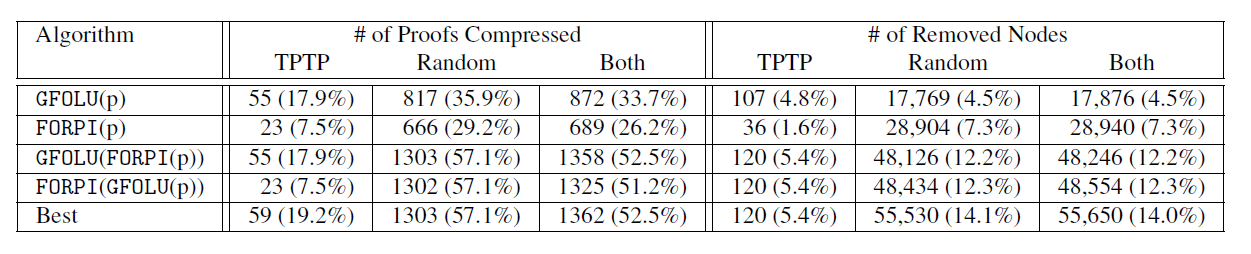
\includegraphics[scale=0.5]{images/table1.png}
\end{frame}

\begin{frame}{Results}
\centering
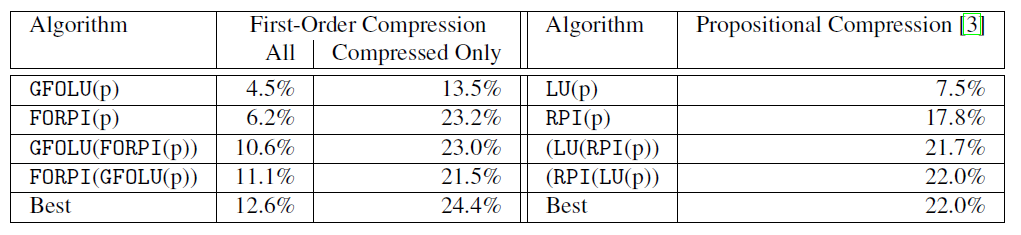
\includegraphics[scale=0.55]{images/table2.png}
\end{frame}


\begin{frame}{Results}
\centering
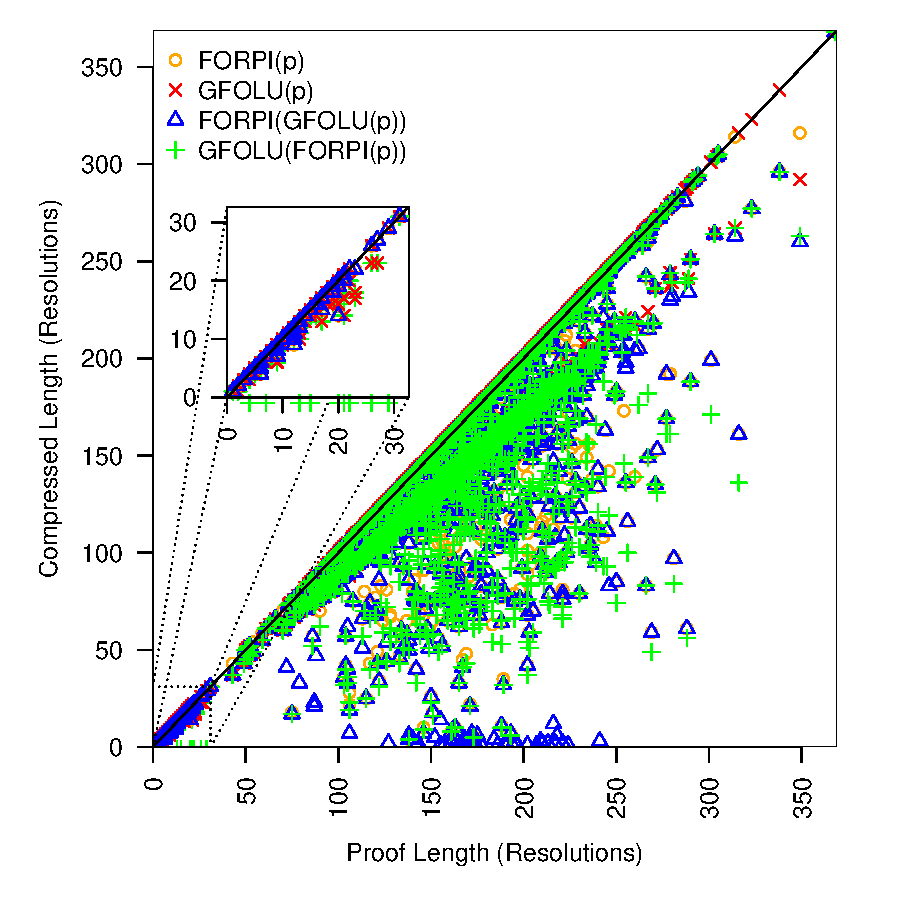
\includegraphics[scale=0.5]{images/combined-all-res-length-vs-compressed-res-length.pdf}
\end{frame}

\begin{frame}{Results}
\centering
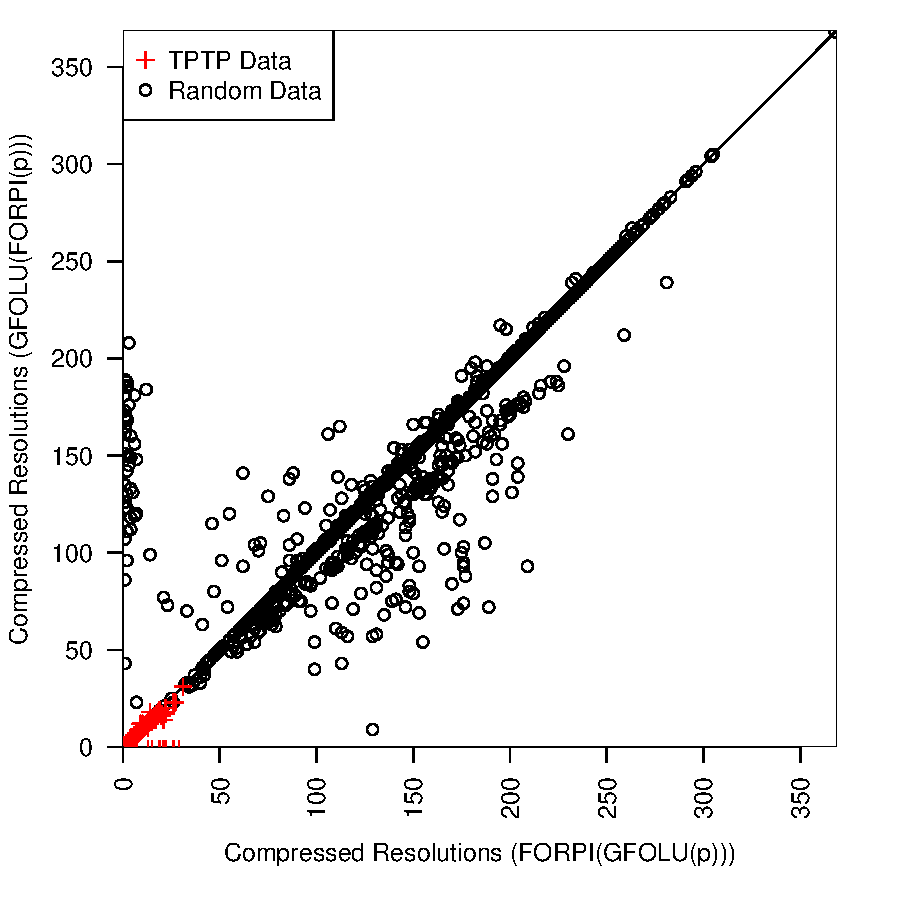
\includegraphics[scale=0.5]{images/combined-alg-res.pdf}
\end{frame}

\begin{frame}{Results}
\centering
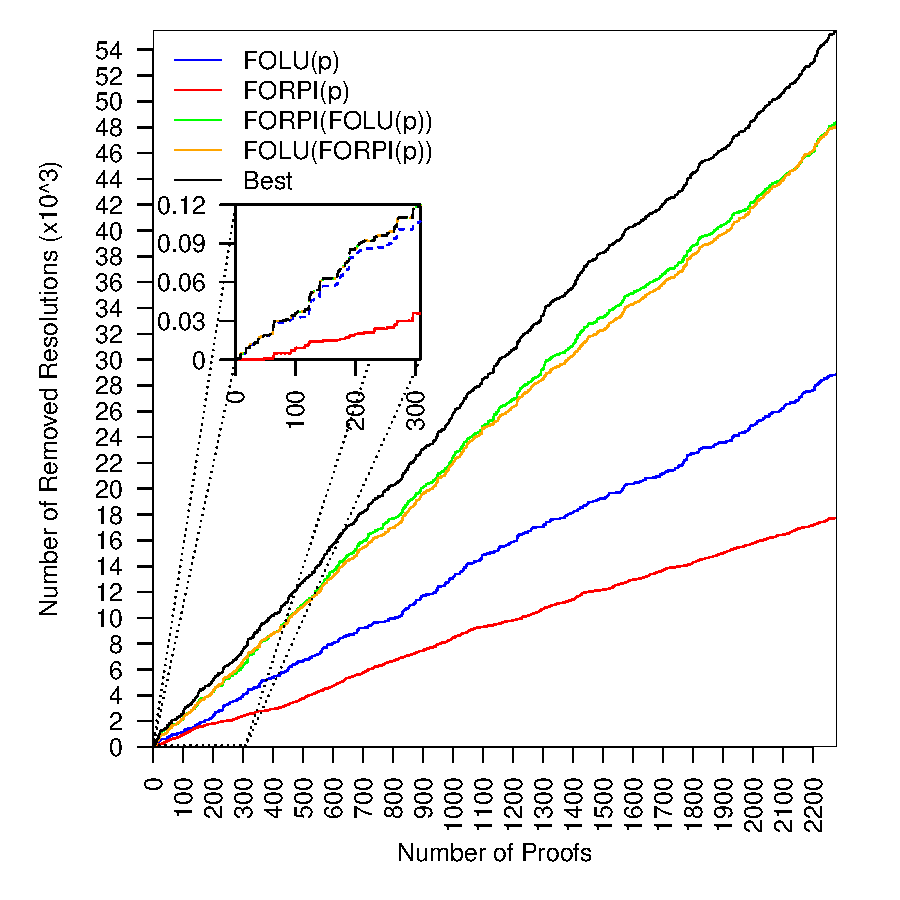
\includegraphics[scale=0.5]{images/combined-all-cumulative-res-nodes-diff.pdf}
\end{frame}






%\section*{Summary}

\begin{frame}{Conclusion}
\begin{itemize}
\item Another simple, quick algorithm lifted from propositional to first-order logic for proof compression. Use both!
\begin{itemize}
\item LowerUnits compresses more often
\item RPI compresses more
\end{itemize}
\item Future work:
\begin{itemize}
\item Explore other proof compression algorithms?
\item Explore ways of dealing with the post-deletion property quickly
\end{itemize}
\end{itemize}



\begin{center}
\alert{Thank you for your attention.\\
Any questions?}
\end{center}
\footnotesize{
\begin{itemize}
\item Source code: \url{https://github.com/jgorzny/Skeptik}
\item Data: \url{https://cs.uwaterloo.ca/~jgorzny/data/}
\item Expanded paper on Arxiv!
\end{itemize}
}
\end{frame}

\begin{frame}[allowframebreaks]{References}
        \bibliographystyle{amsalpha}
\bibliography{ref.bib}
\end{frame}

\begin{frame}{To-do}
\begin{scriptsize}
\begin{prooftree}
\def\e{\mbox{\ $\vdash$\ }}
\AxiomC{$\eta_8$: $p(X),q(X),r(X)\e$}
\AxiomC{$\eta_7$: $\e p(Y)$}
\BinaryInfC{$\eta_6$: $q(Y),r(Y)\e$}
\AxiomC{$\eta_5$: $p(Z) \e q(Z)$}
\BinaryInfC{$\eta_4$: $p(Z),r(Z)\e$}
\AxiomC{$\eta_3$: $\e r(W)$}
\BinaryInfC{$\eta_2$: $p(W)\e$}
\AxiomC{\hspace{-2cm}$\eta_1$: $\e p(U)$}
\BinaryInfC{$\psi$: $\bot$}
\end{prooftree}
\end{scriptsize}
\end{frame}


\end{document}


